We turn to \stage{5}\ in \fref{algorithm}.
It can be seen in, for example, \eref{pc-example} that the surrogate model has a negligibly small computational cost at this stage: for any outcome of the parameters $\vZ \equiv \vZ(\o)$, we can easily compute the corresponding temperature by plugging in $\vZ$ into \eref{pc-example}; the same applies to power.
Hence, the constructed representation can be trivially analyzed to retrieve various statistics about the system in \eref{fourier-system}.
Let us illustrate a few of them still retaining the example in \eref{pc-example}.
Assume that the dynamic power profile $\profilePdyn$ corresponding to the considered workload is the one shown in \fref{application-power}.
Having constructed the surrogate with respect to this profile, we can then rigorously estimate, say, the \pdf\ of temperature at some $k$th moment of time by sampling the surrogate and obtain curves similar to those shown \fref{experimental-results-pdf} (discussed in \sref{experimental-results}).
Furthermore, the expectation and variance of temperature are trivially calculated using the formulae in \eref{pc-moments} where $\pcterms = 6$.
For the whole time span of the power profile $\profilePdyn$ depicted in \fref{application-power}, these quantities are plotted in \fref{application-temperature}.
The displayed curves closely match those obtained via MC simulations with $10^4$ samples; however, our method takes less than a second whilst MC sampling takes more than a day as we shall see next.
\begin{figure}
  \centering
  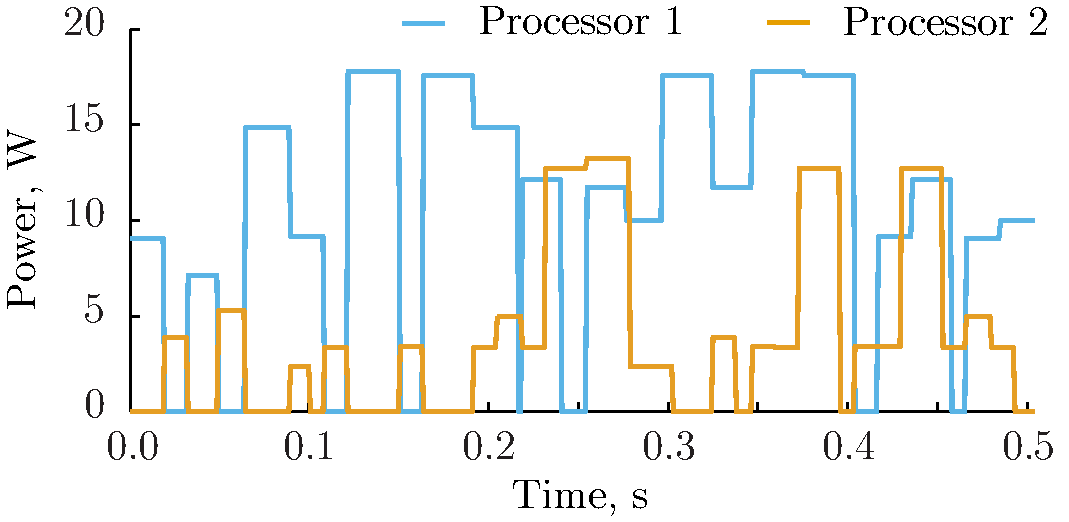
\includegraphics[width=1.00\columnwidth]{include/assets/application-power.pdf}
  \vspace{-0.5em}
  \caption{A dynamic power profile.}
  \flabel{application-power}
  \vspace{-0.5em}
\end{figure}

\begin{figure}[bl]
  \vspace{-1.0em}
  \centering
  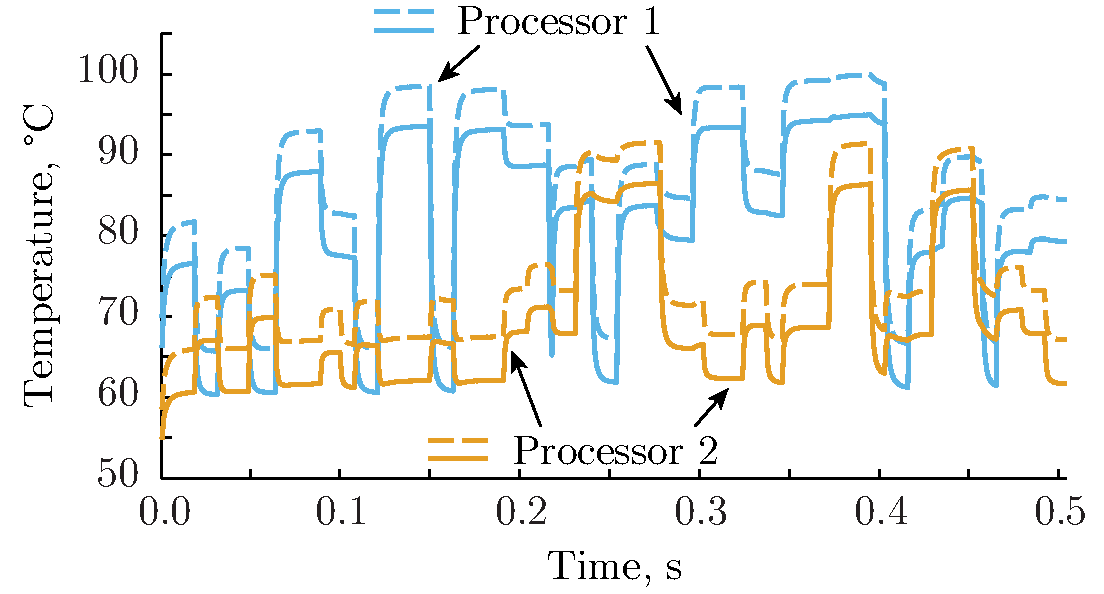
\includegraphics[width=0.90\columnwidth]{include/assets/application-temperature.pdf}
  \vspace{-0.5em}
  \caption{The expected temperature (the solid lines) and one standard deviation above it (the dashed lines).}
  \flabel{application-temperature}
\end{figure}

